\section{Vorbereitungsfragen}
\label{sec:Vorbereitungsfragen}

\subsection{Beschreiben Sie kurz Aufbau und Wirkungsweise der Brennstoffzelle am Beispiel der PEMFC}
In \autoref{fig:230618_PEMFC_Aufbau} ist der Aufbau einer üblichen PEM-Brennstoffzelle veranschaulicht. 
Eine PEMFC ist eine Brennstoffzelle, die Wasserstoff und Sauerstoff in elektrische Energie umwandelt.
Dabei wird Wasserstoff auf der Anode oxidiert und gibt dabei Elektronen ab.
Die Wasserstoffprotonen wandern durch die Membran zur Kathode.
Die Elektronen fließen durch einen äußeren Stromkreis und erzeugen dabei elektrische Energie.
An der Kathode werden die Elektronen mit den Wasserstoffprotonen und Sauerstoff Atomen reduziert und Bilden Wasser.

\begin{figure}[H]
    \centering
    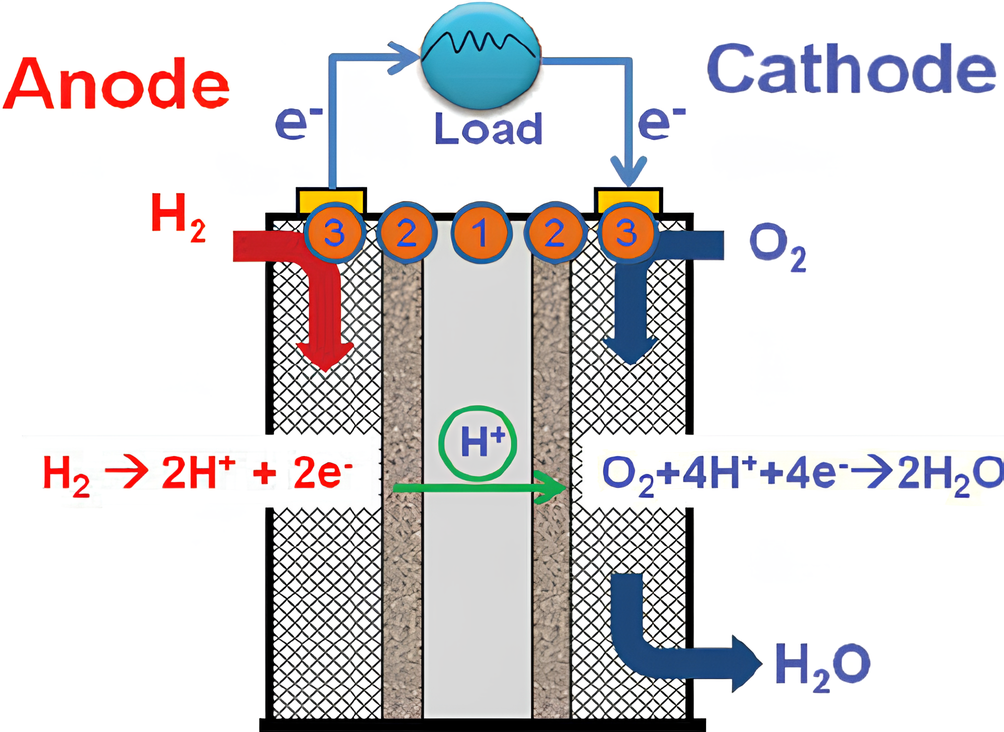
\includegraphics[width=0.5\textwidth]{Abbildungen/PEMFC_Aufbau.png}
    \caption{Aufbau und Funktionsweise einer PEMFC \cite{PEMFC}}
    \label{fig:230618_PEMFC_Aufbau}
\end{figure}

\subsection{Nennen Sie Ausführungsformen von Brennstoffzellen, systematisiert nach der Arbeitstemperatur}

\begin{table}[H]
    \caption{Ausführungsformen von Brennstoffzellen}
    \centering
        \begin{tabular}[pos]{|c|c|c|c|c|c|}
            \hline
            \rowcolor[HTML]{70AD47} 
            BZ-Typen    & Elektrolyt                        & Brennstoff                        & Oxidator                  & Arbeitstemp.          & $\eta$            \\
            \rowcolor[HTML]{70AD47} 
                        &                                   & (Anode)                           & Kathode                   & in °C                 &                   \\\hline\hline
            AFC         & 30\%'ige                          & nur reinst                        & nur reinst                & 60 - 80               & $70 - 75\%$       \\
                        & KOH-Lauge                         & $H_2$                             & $O_2$                     &                       &                   \\\hline
            PEMFC       & PEM (z.B. Nafion)                 & $H_2$,                            & $O_2$, Luft               & 70 - 90               & $40 - 50\%$       \\
                        &                                   & Reformat gas                      &                           &                       &                   \\\hline
            DMFC        & PEM (z.B. Nafion)                 & $CH_3OH$                          & $O_2$, Luft               & 60 - 120              & $40\%$            \\\hline
            PAFC        & Phosphorsäure                     & $H_2$, $CH_4$,                    & $O_2$, Luft               & 170 - 200             & $40 - 50\%$       \\
                        &                                   & Sondergase                        &                           &                       &                   \\\hline
            MCFC        & Akalicarbonat-                    & $H_2$, Erdgase                    & $O_2$, Luft               & 650                   & $55 - 60\%$       \\
                        & schmelzen                         & Sondergase                        &                           &                       &                   \\\hline
            SOFC        & Ytriumdotiertes-                  & $H_2$, Erdgas,                    & $O_2$, Luft               & 900 - 1000            & $60 - 70\%$       \\
                        & zirkonoxod                        & Sondergase                        &                           &                       &                   \\\hline
        \end{tabular}
        \label{tab:20230618_BZ-arten}
\end{table}

\subsection{Skizzieren Sie qualitativ die U-I-Kennlinie einer Brennstoffzelle und erläutern Sie Arbeitsbereiche und markante Betriebsparameter}

\begin{figure}[H]
    \centering
    \includegraphics[width=0.8\textwidth]{Abbildungen/U-I-Kennlinie.png}
    \caption{U-J Kennlinie einer Brennstoffzelle vgl. \cite{BZ-Folien}}
    \label{fig:230618_U-I-Kennlinie}
\end{figure}

In \autoref{fig:230618_U-I-Kennlinie} ist eine Skizze der U-J Kennlinie einer Brennstoffzelle zu erkennen.
Durch die Proportionalität zwischen Stromdichte und der Stromstärke ist das qualitative aussehen der U-I und der U-J Kennlinie deckungsgleich.
Die maskierten Bereiche unterscheiden sich jeweils durch die vorherrschenden Verluste.
In Bereich 1 sind die Aktivierungsverluste maßgeblich, da eine Energiebarriere der Reaktion überwunden werden muss.
Im 2. Bereich dominieren die Ohm'schen Verluste, die aufgrund des Transports der Ionen durch den Elektrolyten und der Elektronen durch das Elektrodenmaterials auftreten.
Im Bereich 3 wird die Reaktion durch die Diffusionsfähigkeit der Gase und der Elektrodenstruktur bestimmt.

\subsection{Wiederholen Sie kurz die Faraday'schen Gesetze.}

\subsubsection{1. Faraday'sches Gesetz}

Die Stoffmenge($n$), die an einer Elektrode während der Elektrolyse abgeschieden wird, ist proportional zur Ladung($Q$), die durch den Elektrolyten geschickt wird \cite{Faraday_G} und beschreibt somit die \autoref{eq:230618_1FaradayGesetz}.
Durch Erweiterungen wird es heutzutage wie in \autoref{eq:230618_1FaradayGesetz_Heute} Formuliert.

\begin{equation}
    n \sim Q
    \label{eq:230618_1FaradayGesetz}
\end{equation}

\begin{equation}
    Q = n \cdot z \cdot F
    \label{eq:230618_1FaradayGesetz_Heute}
\end{equation}

\subsubsection{2. Faraday'sches Gesetz}

Die durch eine bestimmte Ladung abgeschiedene Masse eines Elements ist proportional zum Atomgewicht des abgeschiedenen Elements und umgekehrt proportional zu seiner Wertigkeit, daher zur Anzahl von einwertigen Atomen, die sich mit diesem Element verbinden können \cite{Faraday_G} und formuliert die \autoref{eq:230618_2FaradayGesetz}.
Heutzutage wird das 2. Faraday'sche Gesetz mit \autoref{eq:230618_2FaradayGesetz_Heute} Formuliert.

\begin{equation}
    m \sim \frac{M}{z}
    \label{eq:230618_2FaradayGesetz}
\end{equation}

\begin{equation}
    m = M \cdot n = \frac{M \cdot Q}{z \cdot F} = \frac{M \cdot I \cdot t}{z \cdot F}
    \label{eq:230618_2FaradayGesetz_Heute}
\end{equation}

\subsection{Leiten Sie aus dem Faraday'schen Gesetz eine Gleichung für den Umsatzwirkungsgrad her.}

Der Faraday'sche Wirkungsgrad lässt sich nach \autoref{eq:230618_Faraday-Wirkungsgrad} aus dem Quotienten von theoretisch benötigtem Wasserstoffvolumen und dem tatsächlich benötigtem gemessenen verbrauchtem Wasserstoff ermitteln.
Das theoretisch benötigte Wasserstoffvolumen lässt sich mittels \autoref{eq:230618_Volumen-H2-Theoretisch} berechnen.

\begin{equation}
    \eta_{Theor.} = \frac{V_{Theoretisch(H_2)}}{V_{Praktisch(H_2)}}
    \label{eq:230618_Faraday-Wirkungsgrad}
\end{equation}

\begin{equation}
    V_{H_2} = \frac{I \cdot t \cdot V_m}{z \cdot F}
    \label{eq:230618_Volumen-H2-Theoretisch}
\end{equation}